\section{Evaluation}

\begin{frame}
	\frametitle{Evaluation techniques}
	
	\vspace{0.3cm}
	
	\begin{center}
		\begin{tikzpicture}
			\node at (0,0) [draw=white,ultra thick,inner sep=0pt] {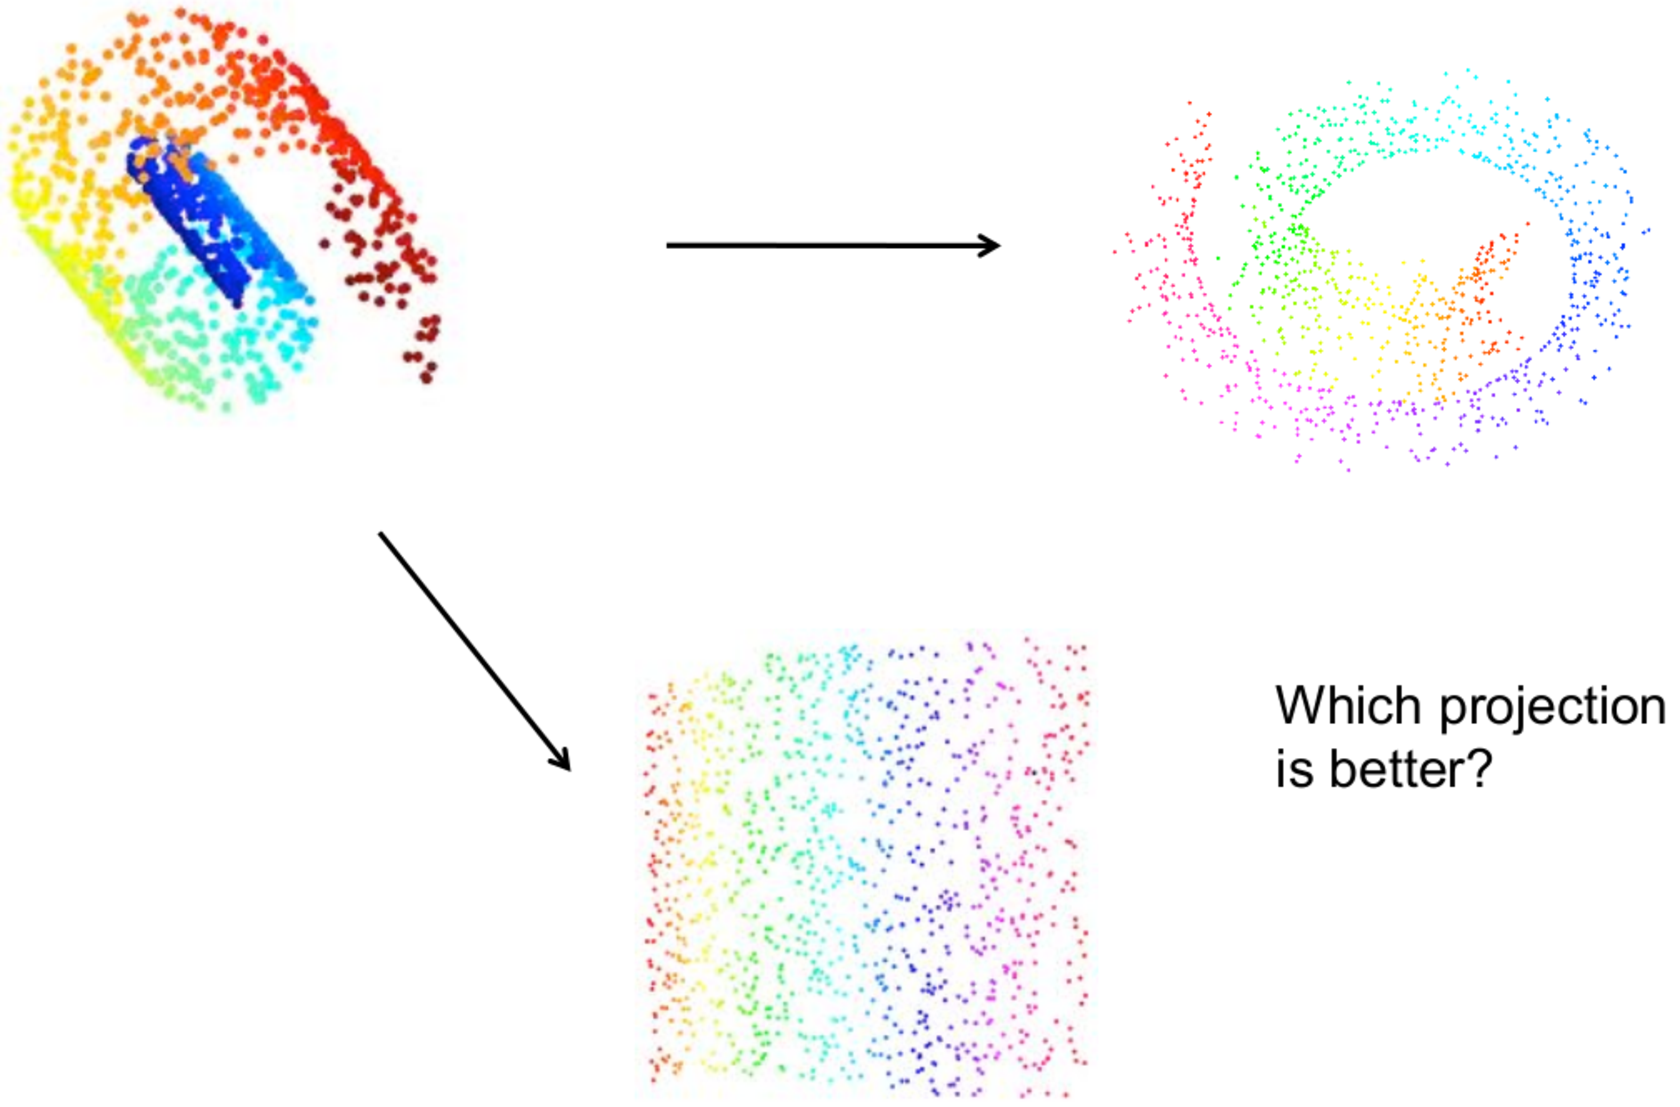
\includegraphics[scale=0.37]{Figures/Evaluation1}};
		\end{tikzpicture}
	\end{center}
\end{frame}

\begin{frame}
	\frametitle{Evaluation techniques}
	
	Evaluation techniques are necessary for:
	
	\vspace{0.1cm}
	
	\begin{itemize}
		\item comparison of methods
		\item scientifically valid and easy evaluation
		\item quality check for the user
		\item ...
	\end{itemize}
\end{frame}

\begin{frame}
	\frametitle{k-NN evaluation}
	
	\begin{tabbing}
		\hspace*{0.35cm}
		Original data set
		\hspace*{4.85cm}
		Projected data set
	\end{tabbing}
	
	\begin{center}
		\begin{tikzpicture}
			\node at (0,0) [draw=white,ultra thick,inner sep=0pt] {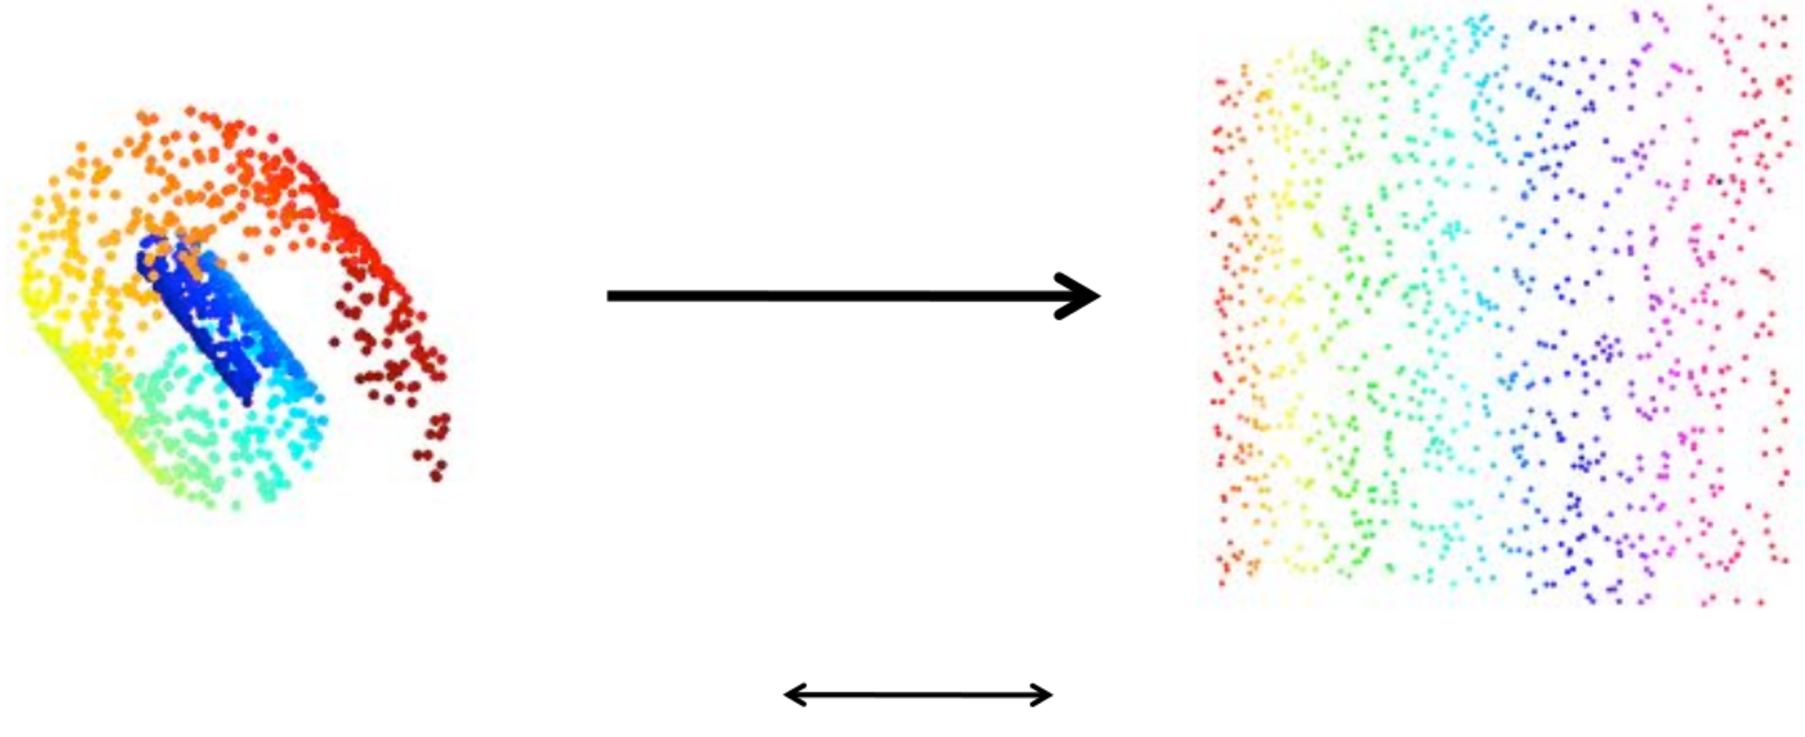
\includegraphics[scale=0.37]{Figures/Evaluation2}};
		\end{tikzpicture}
	\end{center}
	
	\vspace{-1.53cm}
	
	\begin{tabbing}
		\hspace*{0.13cm}
		determine k-NN error
		\hspace*{4.1cm}
		determine k-NN error
	\end{tabbing}
\end{frame}

\begin{frame}
	\frametitle{k-NN evaluation}
	
	\begin{center}
		\begin{tikzpicture}
			\node at (0,0) [draw=white,ultra thick,inner sep=0pt] {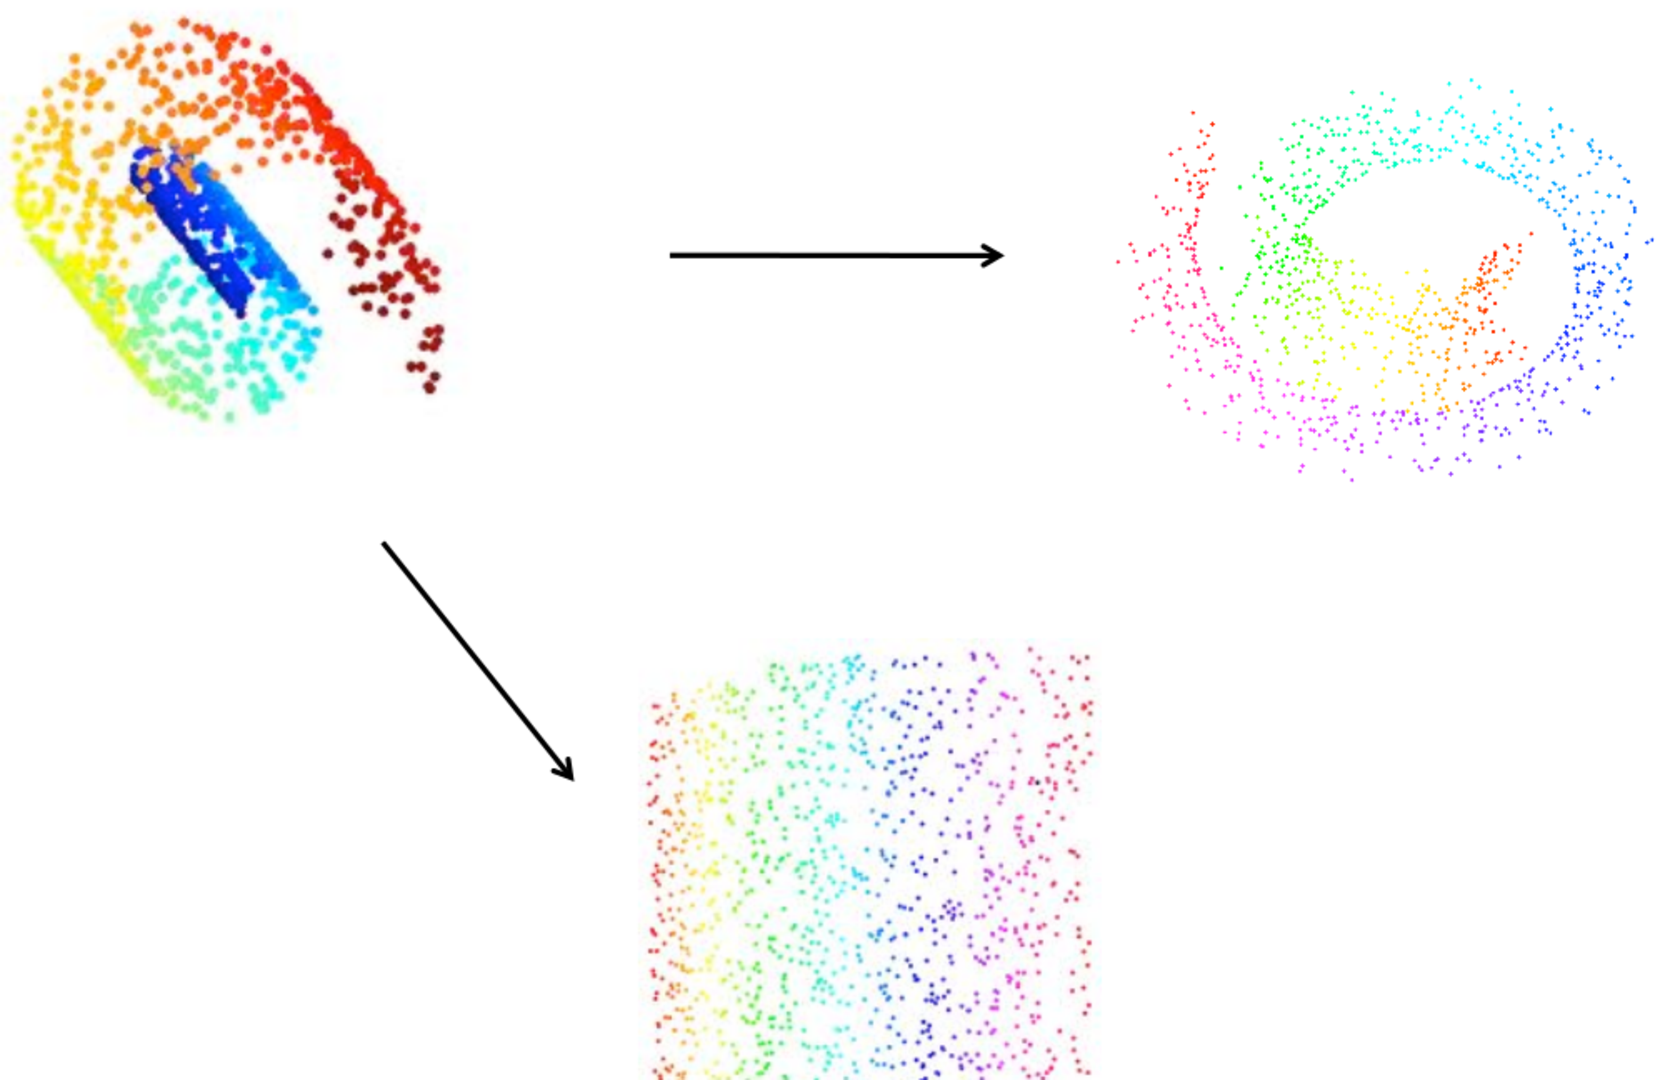
\includegraphics[scale=0.33]{Figures/Evaluation3}};
		\end{tikzpicture}
	\end{center}
	
	\vspace{-7.5cm}
	
	\begin{tabbing}
		\hspace*{0.7cm}
		1-NN accuracy: 0.94
	\end{tabbing}
	
	\vspace{-1.2cm}
	
	\begin{tabbing}
		\hspace*{7.1cm}
		1-NN accuracy: 0.914
	\end{tabbing}
	
	\vspace{3.7cm}
	
	\begin{tabbing}
		\hspace*{7.7cm}
		1-NN accuracy: 0.936
	\end{tabbing}
\end{frame}
